\hypertarget{rate-user}{%
\subsection{Rate User}\label{rate-user}}

\hypertarget{ux3c0ux3b5ux3c1ux3b9ux3b3ux3c1ux3b1ux3c6ux3ae}{%
\subsubsection{Περιγραφή}\label{ux3c0ux3b5ux3c1ux3b9ux3b3ux3c1ux3b1ux3c6ux3ae}}

Ο χρήστης επιθυμεί να βαθμολογήσει έναν άλλο χρήστη.

\hypertarget{ux3b2ux3b1ux3c3ux3b9ux3baux3ae-ux3c1ux3bfux3ae}{%
\paragraph{Βασική
Ροή}\label{ux3b2ux3b1ux3c3ux3b9ux3baux3ae-ux3c1ux3bfux3ae}}

\begin{enumerate}
\def\labelenumi{\arabic{enumi}.}
\tightlist
\item
  Ο χρήστης επιλέγει ``Rate'' στην οθόνη User Details.
\item
  Το σύστημα ελέγχει αν υπάρχει ήδη βαθμολογία στο προφίλ του
  βαθμολογούμενου.
\item
  Η εφαρμογή εμφανίζει την φόρμα βαθμολόγησης στην οθόνη Rate User.
\item
  Ο χρήστης επιλέγει την βαθμολογία που θεωρεί και προσθέτει σχόλια στην
  οθόνη Rate User.
\item
  Το σύστημα εμφανίζει τον διάλογο επιβεβαίωσης βαθμολογίας.
\item
  Ο χρήστης επιλέγει ``Confirm'' στον διάλογο επιβεβαίωσης.
\item
  Το σύστημα καταχωρεί την βαθμολογία στο προφίλ του βαθμολογούμενου.
\item
  Το σύστημα υπολογίζει τη νέα συνολική βαθμολογία του βαθμολογούμενου.
\item
  Το σύστημα εμφανίζει μήνυμα επιτυχίας στην οθόνη User Details.
\end{enumerate}

\hypertarget{ux3b5ux3bdux3b1ux3bbux3bbux3b1ux3baux3c4ux3b9ux3baux3ae-ux3c1ux3bfux3ae-ux3bf-ux3c7ux3c1ux3aeux3c3ux3c4ux3b7ux3c2-ux3adux3c7ux3b5ux3b9-ux3b4ux3ceux3c3ux3b5ux3b9-ux3b2ux3b1ux3b8ux3bcux3bfux3bbux3bfux3b3ux3afux3b1}{%
\paragraph{Εναλλακτική Ροή: Ο χρήστης έχει δώσει
βαθμολογία}\label{ux3b5ux3bdux3b1ux3bbux3bbux3b1ux3baux3c4ux3b9ux3baux3ae-ux3c1ux3bfux3ae-ux3bf-ux3c7ux3c1ux3aeux3c3ux3c4ux3b7ux3c2-ux3adux3c7ux3b5ux3b9-ux3b4ux3ceux3c3ux3b5ux3b9-ux3b2ux3b1ux3b8ux3bcux3bfux3bbux3bfux3b3ux3afux3b1}}

\begin{enumerate}
\def\labelenumi{\arabic{enumi}.}
\setcounter{enumi}{2}
\tightlist
\item
  H εφαρμογή εμφανίζει μήνυμα ήδη υπάρχουσας βαθμολογίας στην οθόνη User
  Details.
\end{enumerate}

\hypertarget{ux3b5ux3bdux3b1ux3bbux3bbux3b1ux3baux3c4ux3b9ux3baux3ae-ux3c1ux3bfux3ae-ux3b1ux3baux3cdux3c1ux3c9ux3c3ux3b7}{%
\paragraph{Εναλλακτική Ροή:
Ακύρωση}\label{ux3b5ux3bdux3b1ux3bbux3bbux3b1ux3baux3c4ux3b9ux3baux3ae-ux3c1ux3bfux3ae-ux3b1ux3baux3cdux3c1ux3c9ux3c3ux3b7}}

\begin{enumerate}
\def\labelenumi{\arabic{enumi}.}
\setcounter{enumi}{5}
\tightlist
\item
  Ο χρήστης επιλέγει ``Cancel'' στον διάλογο επιβεβαίωσης.
\item
  Το σύστημα επιστρέφει στην οθόνη User Details.
\end{enumerate}

\hypertarget{ux3b1ux3bdux3acux3bbux3c5ux3c3ux3b7-ux3b5ux3c5ux3c1ux3c9ux3c3ux3c4ux3afux3b1ux3c2}{%
\subsubsection{Ανάλυση
Ευρωστίας}\label{ux3b1ux3bdux3acux3bbux3c5ux3c3ux3b7-ux3b5ux3c5ux3c1ux3c9ux3c3ux3c4ux3afux3b1ux3c2}}

\begin{figure}
\centering
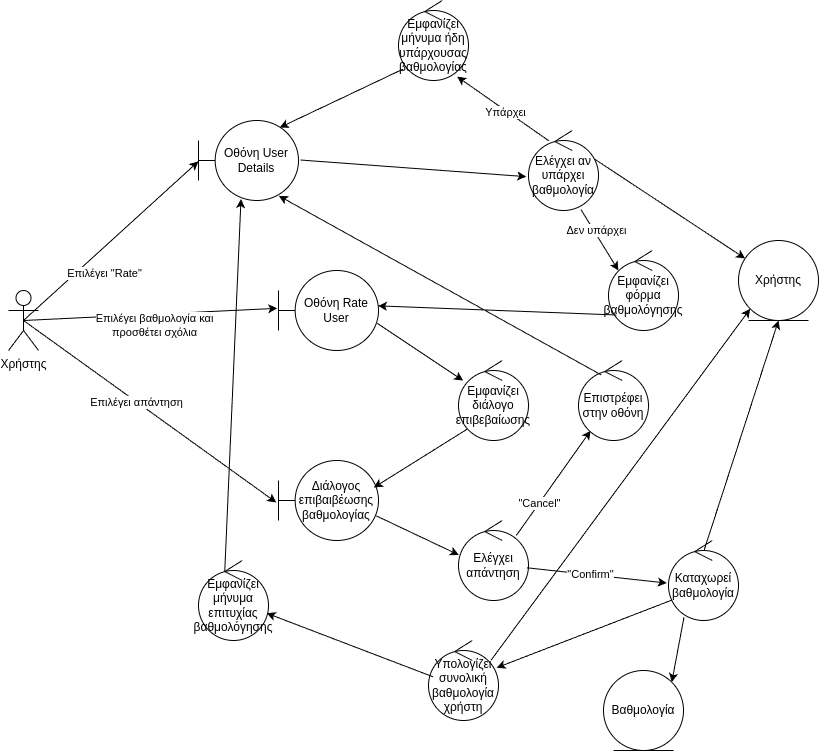
\includegraphics{./rate-user-robustness.drawio.png}
\caption{image}
\end{figure}
